\documentclass[french]{article}
\usepackage[utf8x]{inputenc}
\usepackage[T1]{fontenc}
\usepackage{babel}
\usepackage{lmodern}
\usepackage[top=2cm,bottom=2cm,left=3cm,right=3cm]{geometry}
\usepackage{microtype}
\usepackage{mathtools, amssymb, amsthm}
\usepackage{mdframed}
\usepackage{hyperref}
\usepackage{graphicx}
\usepackage{xcolor}
\usepackage{mathrsfs}
\usepackage{wrapfig}
\usepackage{stmaryrd}
\usepackage{dsfont}
\usepackage{framed}

\newtheorem{prototheorem}{Théorème}[section]
\newenvironment{thm}
   {\colorlet{shadecolor}{red!7}\begin{shaded}\begin{prototheorem}}
   {\end{prototheorem}\end{shaded}}

\newtheorem{protocorollary}[prototheorem]{Corollaire}
\newenvironment{corollary}
    {\colorlet{shadecolor}{violet!10}\begin{shaded}\begin{protocorollary}}
    {\end{protocorollary}\end{shaded}}

\newtheorem{protolemma}[prototheorem]{Lemme}
\newenvironment{lemma}
    {\colorlet{shadecolor}{pink!15}\begin{shaded}\begin{protolemma}}
    {\end{protolemma}\end{shaded}}

\newtheorem{protodefinition}{Définition}[section]
\newenvironment{definition}
    {\colorlet{shadecolor}{green!5}\begin{shaded}\begin{protodefinition}}
    {\end{protodefinition}\end{shaded}}

\newtheorem{protoproposition}{Proposition}[section]
\newenvironment{prop}
    {\colorlet{shadecolor}{blue!5}\begin{shaded}\begin{protoproposition}}
    {\end{protoproposition}\end{shaded}}


\newtheorem*{remark}{Remarque}
\newtheorem{exo}{Exercice}
\newtheorem*{exemple}{Exemple}


\newcommand{\lesss}{\rotatebox[origin=c]{90}{$\land$}}
\newcommand{\less}{\ \lesss\ }

\newcommand{\biggg}{\rotatebox[origin=c]{90}{$\lor$}}
\newcommand{\bg}{\ \biggg\ }

\title{\bsc{Théorie des représentations}}
\date{\today}
\author{Anastasiia \bsc{Chernetcova}}

\begin{document}

\maketitle

\tableofcontents

%Vous devez m'envoyer un fichier .tex (et éventuellement un fichier avec une image) que je peux compiler en un document pdf de 4 à 5 pages. Il est important dans votre fichier .tex que vous utilisiez :
%- une table des matières, (OK)
-% des références (labels), (OK)
%- au moins une liste (OK)
%- des commandes personnelles,
%- des commandes mathématiques,
%- au moins une image (importée ou créée avec Tikz), (OK)
%- une bibliographie.

\section{Prérequis}

\subsection{Action de groupe sur un ensemble}

\begin{definition}[Action à gauche]

  Une action (à gauche) d'un groupe \(G\) sur un ensemble \(X\) est une application
  \[\begin{matrix}
  \psi : & G \times X & \longrightarrow & X \\
  \ & (g,x) & \longmapsto & g \cdot x
  \end{matrix}\]

  telle que :

  \begin{enumerate}
    \item \(\forall x \in X, e \cdot x = x\) (où \(e\) est l'élément neutre de \(G\)) ;
    \item \(\forall g, h \in G, \forall x \in X, g \cdot (h \cdot x) = (gh) \cdot x\).
  \end{enumerate}

  On dit alors que \(G\) agit sur \(X\).
\end{definition}

\begin{prop}
  Si un groupe \(G\) agit sur \(X\) par \(\begin{matrix}
   G \times X & \longrightarrow & g \cdot x \\
   (g,x) & \longmapsto & g \cdot x
  \end{matrix}\), alors pour tout \(g \in G\), l'application

  \[ \begin{matrix}
  \pi_g : & X & \longrightarrow & X \\
  \ & x & \longmapsto & g \cdot x
  \end{matrix}\]

   est une permutation de \(X\), et l'application

   \[\begin{matrix}
   \pi : & G & \longrightarrow & \mathfrak{S}_{X}  \\
   \ & g & \longmapsto & \pi_g
   \end{matrix}\] est un morphisme de groupes.

   La réciproque est aussi vraie.

   Cela établit deux bijections réciproques entre l'ensemble des actions de \(G\) sur \(X\) et celui des morphismes de \(G\) dans \(\mathfrak{S}_{X} \).

\end{prop}

\begin{remark}[Notations]
  On note \(\mathfrak{S}_n\) le groupe symétrique à \(n\) éléments.
\end{remark}

\subsection{Orbites, actions transitive et fidèle, noyau}

\begin{definition}
  Si un groupe \(G\) agit sur \(G\) et si  \(x,y \in X\), on définit la relation \(x R y\) si et seulement si il existe \(g \in G, y = g \cdot x\). \(R\) est une relation d'équivalence.

  La classe d'équivalence de \(x \in X\) pour cette relation s'appelle \textbf{orbite} de \(x\) :

  \begin{equation}\label{fidele}
    \operatorname{Orb}(x) = \{ g \cdot x, g \in G \}.
  \end{equation}

  Ainsi, l'ensemble des orbites forme une partition de \(X\).

  On dit que l'action est \textbf{transitive} ou que \(G\) agit transitivement sur \(X\) s'il n'y a qu'une seule orbite.

  Le \textbf{noyau de l'action} est le noyau du morphisme
  \(\begin{matrix}
  \pi : & G & \longrightarrow & \mathfrak{S}_{X}  \\
  \ & g & \longmapsto & \pi_g
  \end{matrix}\) associé, i. e. l'ensemble

  \[\operatorname{Ker}(\pi) \stackrel{\text{déf.}}{=} \{ g \in G \mid \forall x \in X, g \cdot x = x \}. \]

  On dit que l'action est \textbf{fidèle} ou que $G$ agit \textbf{fidèlement} si le morphisme $\pi$ associé à l'action est injectif, ie si son noyau esr réduit à l'élement neutre.
\end{definition}


\begin{exemple}
  Le groupe \(G = SO(3)\) des rotations de \(\mathbb{R}^3\) de centre \(O\) agit sur l'ensemble \(\mathbb{R}^3\). Les orbites de cette action sont des sphères centrées en l'origine. L'action n'est pas transitive. L'action est fidèle, car la seule rotation fixant tous les points de \(\mathbb{R}^3\) est l'identité.

  \begin{figure}[h!]
    \centering
    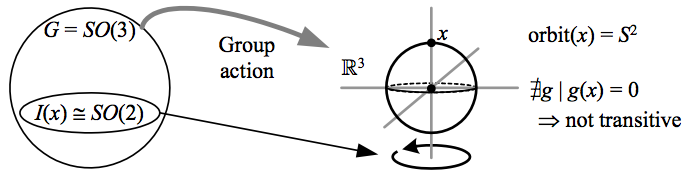
\includegraphics[scale=0.5]{action-groupe-rotation.png}
    \caption{L'action de \(G\) n'est pas transitive. En particulier, il n'existe pas de rotation \(r\) telle que \(\forall x \in \mathbb{R}^3, r(x) = O.\) }
    \label{action-groupe-rotation}
  \end{figure}
\end{exemple}

\subsection{Théorème de Lagrange}

\begin{thm}[De Lagrange] \label{lagrange}
  Soit \(G\) un groupe fini et \(H\) un sous-groupe de \(G\). Alors l'ordre de \(H\) divise celui de \(G\). En particulier, l'ordre d'un élément de \(G\) divise celui de \(G\).
\end{thm}

\section{Représentations linéaires des groupes finis}

\subsection{Représentations, représentations isomorphiques, représentations irréductibles}

La théorie des représentations a été introduite par Georg Frobenius (\ref{Frobenius}) au \textsc{xix}\ieme ~siècle.

\begin{figure}[h!]
  \centering
  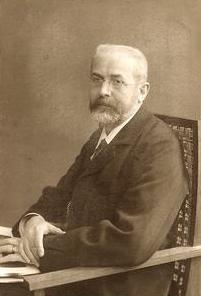
\includegraphics[scale=0.3]{Frobenius.jpg}
  \caption{Georg Frobenius}
  \label{Frobenius}
\end{figure}

\begin{definition}
  Une représentation linéaire d'un groupe \(G\) est la donnée d'un \(\mathbb{C}\)-espace vectoriel \(V\) muni d'une action de groupes (à gauche) de \(G\) agissant de manière \textbf{linéaire} :

  \[\begin{matrix}
    G \times V & \longrightarrow & V \\
    (g,x) & \longmapsto & g \cdot x
  \end{matrix}\]
  %  \begin{array}{rcl}
  %  G \times V & \longrightarrow & V \\
  %  (g,x) & \longmapsto g \cdot x
  %  \end{array}

  telle que

  \begin{enumerate}
    \item \(\forall x \in V, e \cdot x = e\);
    \item \(\forall g, g' \in G, \forall x \in V, g \cdot (g' \cdot x) = (gg')\cdot x\) ;
    \item \(\forall g \in G, \forall x, y \in V, \forall \lambda, \mu \in \mathbb{C}, g \cdot (\lambda x + \mu y) = \lambda g \cdot x+ \mu g \cdot y \).
  \end{enumerate}
\end{definition}

\begin{remark}
  Les deux premières propriétés proviennent du fait que la représentation linéaire est une \textbf{action de groupe} \(G\) et la dernière du fait que c'est une action \textbf{linéaire}.
\end{remark}

%ъуъ

\begin{definition}[Divers]
  L'espace vectoriel \(V\) est appelé \textbf{l'espace de la représentation}.

  La dimension de \(V\) (en tant que \(\mathbb{C}\)-espace vectoriel) est appelé le \textbf{degré} ou la dimension de la représentation.

  Lorsque \(\rho\) est injectif, la représentation est dite \textbf{fidèle}. Le groupe \(G\) se représente alors de manière concrète comme un sous-groupe de \(GL(V)\). Lorsque \(V\) est de dimension finie (ce que nous allons supposer dorénavant), le choix d'une base du \(\mathbb{C}\)-espace vectoriel \(V\) fournit alors une représentation encore plus concrète comme groupe de matrices. En effet, si \(V \simeq \mathbb{C}^{n} \text{ et } \operatorname{dim}(V) = n, \text{ alors } GL(V) \simeq GL_n(\mathbb{C})\), \textbf{le groupe des matrices inversibles} à coefficients dans \(\mathbb{C}\).
\end{definition}

\begin{remark}[Personnelle]
  Si \(\rho\) est une représentation fidèle, alors, si on se réfère à la définition \ref{fidele}, on peut alors écrire :

  \[\operatorname{Ker}(\rho) = \{ g \in G \mid \forall x \in V, g \cdot x = x \} = \{ e \}. \]
\end{remark}

\begin{exemple}

  \

  \begin{enumerate}
    \item \emph{La représentation triviale.}

    \[\begin{matrix}
    \rho : & G & \longrightarrow & GL(\mathbb{C}) \\
    \ & g & \longmapsto & \rho_g = \left(\operatorname{id} :\begin{matrix}
    \mathbb{C} & \longrightarrow & \mathbb{C} \\
    x & \longmapsto & x
    \end{matrix}\right).
    \end{matrix}\]

    \item \emph{Les représentations de degré 1.} Ce sont des morphismes de groupes

    \[\rho : G \longmapsto \mathbb{C} ^{*}.\]

    En effet, si \(V\) est un \(\mathbb{C}\)-espace vectoriel de dimension 1, alors \(GL(V) \simeq \mathbb{C}^{*}\) puisque les endomorphismes de \(V\) sont des homothéties

    \[\begin{matrix}
    f_{\lambda} : & V & \longrightarrow & V \\
    \ & x & \longmapsto & \lambda x
    \end{matrix}\]

    et

    \[\begin{matrix}
    GL(V) & \longrightarrow & \mathbb{C}^{*} \\
    f _{\lambda} & \longmapsto & \lambda,
    \end{matrix}\]

    l'application qui a une homothétie fait correspondre son rapport, est un isomorphisme de groupes.

    Si \(G\) est fini, alors tout élément de \(G\) est d'ordre fini (par le théorème \ref{lagrange}) et donc, pour tout \(g \in G\), \(\rho_g\) est une racine de l'unité dans \(\mathbb{C}\), et en particulier \(\rho_g\) est un nombre complexe de module 1 :

    \[\lvert \rho_g \rvert=1.\]
  \end{enumerate}
\end{exemple}

\begin{exo}
  Soit \(G\) un groupe fini et soit \(\rho : G \longrightarrow GL(V)\) une représentation (complexe linéaire) de \(G\). Montrer que, pour tout \(g \in G\), l'endomorphisme \(\rho_g\) est diagonalisable.
\end{exo}

\begin{proof}[Correction]
  Supposons que \(\lvert G \rvert = n\). Soit \(g \in G\).

  Par le théorème de Lagrange (cf théorème \ref{lagrange}), l'ordre de \(g\) divise celui de \(G\). Donc \(g^{n} = e\), où \(e\) est l'élément neutre de \(G\). Donc on a \((\rho_g)^{n} = \operatorname{id}_V\), d'où \(\rho_g^{n}-\operatorname{id}_V = 0\). Le polynôme \(X^{n}-1 \) est un polynôme annulateur de \(\rho_g\). Alors le polynôme minimal de \(\rho_g\) divise \(X^{n}-1\). Or \(X ^{n}-1\) n'a que des racines simples, à savoir les racines \(n\)-ièmes de l'unité de \(\mathbb{C}\) :

  \[\left\{ e^{\frac{2 i k \pi}{n}}, k \in \llbracket 0, n-1 \rrbracket \right\}.\]  %\{ 0, \dots, n-1 \} .

  Ainsi le polynôme minimal de \(\rho_g\) est scindé à racines simples. Donc l'endomorphisme \(\rho_g\) est diagonalisable.
\end{proof}

\subsection{Théorème de Maschke}

Définissons tout d'abord la notion de somme directe de représentations.

\begin{definition}
  Soit \(G\) un groupe fini. Soit \(\rho : G \to GL(V)\) et \(\rho' : G \to GL(V')\) deux représentations de \(G\). On définit \textbf{la somme directe} \(\rho\oplus \rho'\) comme le rerésentation de \(G\) associée à l'espace vectoriel \(V \oplus V'\) définie par:

  \begin{equation}
    \begin{matrix}
    \rho \oplus \rho' : & G & \longrightarrow & GL(V\oplus V') \\
    \ & g & \longmapsto & \left((\rho \oplus \rho')g : \begin{matrix}
      V \oplus V' & \longrightarrow & V \oplus V' \\
      v + v' & \longmapsto & \rho_g(v) + \rho'_g(v').
    \end{matrix}\right)
    \end{matrix}
  \end{equation}
\end{definition}

\paragraph{Rappel d'algèbre linéaire}


\begin{thm}[De Maschke]
  Toute représentation linéaire complexe de degré fini est somme directe de représentations irréductibles.
\end{thm}

\begin{lemma}
  Tout sous-espace stable d'une représentation linéaire complexe de degré fini d'un groupe fini admet un supplémentaire stable.
\end{lemma}





\end{document}
